%+++++++++++++++++++++++++++++++++++++++++++++++++++++++++++++++++++++++++++++++
%+++++++++++++++++++++++++++++++++++++++++++++++++++++++++++++++++++++++++++++++
%everything belong to gui: 3D visualization, mouse, keys, ...
%
\mysection{3D graphics visualization}
%
The 3D graphics visualization window is kept simple, but useful to see the animated results of the multibody system.
The graphics output is restricted to a 3D window (renderwindow) into which the renderer draws the visualization state of the \texttt{MainSystem} \texttt{mbs}.

%+++++++++++++++++++++++++++++++++++++++++++++++++++++++
%+++++++++++++++++++++++++++++++++++++++++++++++++++++++
\mysubsection{Mouse input}
The following table includes the mouse functions. 

\begin{center}
  \footnotesize
  \begin{longtable}{| p{4cm} | p{4cm} | p{8cm} |} 
	\hline
  \bf Button & action & \bf remarks \\ \hline
  \bf left mouse button & move model & keep left mouse button pressed to move the model in the current x/y plane\\ \hline
  \bf left mouse button & select item & mouse click on any node, object, etc.\ to see its basic information in status line; selection is deactivated if mouse coordinates are shown (see button F3) \\ \hline
  \bf right mouse button & rotate model & keep right mouse button pressed to rotate model around current current $X_1$/$X_2$ axes\\
	\bf right mouse button & show item dictionary & [EXPERIMENTAL, must be activated in visualizationSettings.interactive] (short) press and release right mouse button \\ \hline
\hline
  \bf mouse wheel & zoom & use mouse wheel to zoom (on touch screens 'pinch-to-zoom' might work as well) \\ \hline
  \end{longtable}
\end{center}
Note that current mouse coordinates can be obtained via \texttt{SystemContainer.GetCurrentMouseCoordinates()}.
%
\mysubsubsection{6D mouse}
Graphics engines, especially in CAD and finite elements allow input of special 3D or 6D mouse devices.
There is a basic interface for so-called 3D mouse / 6D mouse or space mouse, allowing to map the 6D joystick to translation and rotation,
see \texttt{visualizationSettings.interactive.useJoystickInput} and similar options.
The interface only works, if the device maps 6 coordinates to the joystick input of GLFW (tested with 3DCONNEXION mouse).

%+++++++++++++++++++++++++++++++++++++++++++++++++++++++
%+++++++++++++++++++++++++++++++++++++++++++++++++++++++
\mysubsection{Keyboard input}
The following table includes the keyboard shortcuts available in the window. 

\begin{center}
  \footnotesize
  \begin{longtable}{| p{4cm} | p{4cm} | p{8cm} |} 
	\hline
  \bf Key(s) & action & \bf remarks \\ \hline
  \bf 1,2,3,4 or 5 & visualization update speed & the entered digit controls the visualization update, ranging within 0.02, 0.1 (default), 0.5, 2, and 100 seconds \\ \hline
	%
  %\bf 0 or KEYPAD 0& reset rotation & set rotation such that the scene is oriented in the x/y plane \\ \hline
  \bf CTRL+1 or SHIFT+CTRL+1& change view& set view in 1/2-plane (+SHIFT: view from opposite side) \\ \hline
  \bf CTRL+2 or SHIFT+CTRL+2& change view& set view in 1/3-plane (+SHIFT: view from opposite side) \\ \hline
  \bf CTRL+3 or SHIFT+CTRL+3& change view& set view in 2/3-plane (+SHIFT: view from opposite side) \\ \hline
  \bf CTRL+4 or SHIFT+CTRL+4& change view& set view in 2/1-plane (+SHIFT: view from opposite side) \\ \hline
  \bf CTRL+5 or SHIFT+CTRL+5& change view& set view in 3/1-plane (+SHIFT: view from opposite side) \\ \hline
  \bf CTRL+6 or SHIFT+CTRL+6& change view& set view in 3/2-plane (+SHIFT: view from opposite side) \\ \hline

  \bf A & zoom all & set zoom such that the whole scene is visible \\ \hline
  \bf CURSOR UP, DOWN, ... & move scene& use coursor keys to move the scene up, down, left, and right (use CTRL for small movements)\\ \hline
	%
  \bf C & show/hide connectors & pressing this key switches the visibility of connectors \\ \hline
  \bf CTRL+C & show/hide connector numbers & pressing this key switches the visibility of connector numbers \\ \hline
  %
	\bf B & show/hide bodies & pressing this key switches the visibility of bodies \\ \hline
  \bf CTRL+B & show/hide body numbers & pressing this key switches the visibility of body numbers \\ \hline
  %
	\bf L & show/hide loads & pressing this key switches the visibility of loads \\ \hline
  \bf CTRL+L & show/hide load numbers & pressing this key switches the visibility of load numbers \\ \hline
  %
	\bf M & show/hide markers & pressing this key switches the visibility of markers \\ \hline
  \bf CTRL+M & show/hide marker numbers & pressing this key switches the visibility of marker numbers \\ \hline
  %
	\bf N & show/hide nodes & pressing this key switches the visibility of nodes \\ \hline
  \bf CTRL+N & show/hide node numbers & pressing this key switches the visibility of node numbers \\ \hline
  %
	\bf S & show/hide sensors & pressing this key switches the visibility of sensors \\ \hline
  \bf CTRL+S & show/hide sensor numbers & pressing this key switches the visibility of sensor numbers \\ \hline
  %
	\bf T & faces / edges mode & switch between faces transparent/ faces transparent + edges / only face edges / full faces with edges / only faces visible \\ \hline
  %
	\bf Q & stop solver & current solver is stopped (proceeds to next simulation or end of file) \\ \hline
	%
	\bf X & execute command & open dialog to enter a python command (in global python scope); dialog may appear behind the visualization window! User errors may lead to crash -- be careful! 
	Examples: '\texttt{print(mbs)}', '\texttt{x=5}', '\texttt{mbs.GetObject(0)}',etc.\\ \hline
	%
	\bf V & visualization settings & open dialog to modify visualization settings; dialog may appear behind the visualization window! \\ \hline
	%
	\bf F3 & show mouse coordinates & shown in status line \\ \hline
  \bf ESCAPE & close simulation & stops the simulation (and further simulations) and closes the render window (same as close window) \\ \hline
  \bf SPACE & continue simulation & if simulation is paused, it can be continued by pressing space; use SHIFT+SPACE to continuously activate 'continue simulation'\\ \hline
%
	%\bf F2 & ignore keys &  \\ \hline
  %\bf KEYPAD 2/8,4/6,1/9 & rotate scene & about 1, 2 and 3-axis (use CTRL for small rotations) \\ \hline
  %\bf '.' or KEYPAD + & zoom in & zoom one step into scene (additionally press CTRL to perform small zoom step)\\ \hline
  %\bf ',' or KEYPAD - & zoom out & zoom one step out of scene (additionally press CTRL to perform small zoom step)\\ \hline
  \end{longtable}
\end{center}

Special keys:
\begin{center}
  \footnotesize
  \begin{longtable}{| p{4cm} | p{4cm} | p{8cm} |} 
	\hline
	\bf F2 & ignore keys & ignore all keyboard input, except for KeyPress user function, F2 and escape \\ \hline
  \bf KEYPAD 2/8,4/6,1/9 & rotate scene & about 1, 2 and 3-axis (use CTRL for small rotations) \\ \hline
  \bf '.' or KEYPAD + & zoom in & zoom one step into scene (additionally press CTRL to perform small zoom step)\\ \hline
  \bf ',' or KEYPAD - & zoom out & zoom one step out of scene (additionally press CTRL to perform small zoom step)\\ \hline
  \end{longtable}
\end{center}

%+++++++++++++++++++++++++++++++++++++++++++++++++++++++++++++++++++++++++++++
\mysubsection{GraphicsData}
\label{sec:graphicsData}
All graphics objects are defined by a \texttt{GraphicsData} structure.%, see \refSection{sec:graphicsData}.
Note that currently the visualization is based on a very simple and ancient OpenGL implementation, as there is currently no simple platform independent alternative. However, most of the heavy load triangle-based operations are implemented in C++ and are realized by very efficient OpenGL commands. However, note that the number of triangles to represent the object should be kept in a feasible range ($<1000000$) in order to obtain a fast response of the renderer.

Many objects include a \texttt{GraphicsData} dictionary structure for definition of attached visualization of the object.
Note that objects expect a list of \texttt{GraphicsData}, which can be produced with \texttt{GraphicsData...(...)} functions. Note that if reading out the \texttt{GraphicsData} from the object again, it usually has a different structure sorted by types of \texttt{GraphicsData}.
Typically, you can use primitives (cube, sphere, ...) or \ac{STL} data to define the objects appearance.
\texttt{GraphicsData} dictionaries can be created with functions provided in the utilities module \texttt{exudyn.graphicsDataUtilities.py}, see \refSection{sec:module:graphicsDataUtilities}.

\texttt{GraphicsData} can be transformed into points and triangles (mesh) and can be used for contact computation, as well.
\mybold{NOTE} that for correct rendering and correct contact computations, all triangle nodes must follow a strict local order and triangle normals -- if defined -- must point outwards, see \fig{fig:triangleNormals}.
\begin{figure}[tbh]%
\begin{center}
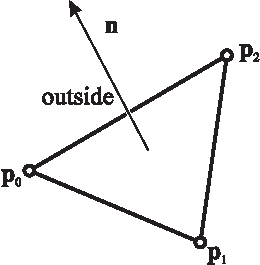
\includegraphics[width=0.25\columnwidth]{figures/triangleNormal}%
\end{center}
\caption{Definition of triangle normals and outside/inside regions in Exudyn: the normal to a triangle with vertex positions $\pv_0$, $\pv_1$, $\pv_2$ is computed from cross product as $\nv = \frac{(\pv_1-\pv_0) \times (\pv_2-\pv_0)}{|(\pv_1-\pv_0) \times (\pv_2-\pv_0)|}$;
the normal $\nv$ then points to the outside region of the mesh or body; the direction of $\nv$ just depends on the ordering of the vertex points (interchange of two points changes the normal direction); correct normals are needed for contact computations as well as for correct shading effects in visualization.}%
\label{fig:triangleNormals}%
\end{figure}

\texttt{BodyGraphicsData} contains a list of \texttt{GraphicsData} items, i.e.\ bodyGraphicsData = [graphicsItem1, graphicsItem2, ...]. Every single \texttt{graphicsItem} may be defined as one of the following structures using a specific 'type':
\begin{center}
  \footnotesize
  \begin{longtable}{| p{3cm} | p{2cm} | p{3cm} | p{7.5cm} |} 
	\hline
  \bf Name & \bf type & \bf default value & \bf description \\ \hline
%
%LINE
	\multicolumn{3}{l}{\parbox{8cm}{\bf type = 'Line': }} & \multicolumn{1}{l}{\parbox{7.5cm}{\it draws a polygonal line between all specified points}}\\ \hline
  color & list & [0,0,0,1] & list of 4 floats to define RGB-color and transparency\\ \hline
  data & list &  mandatory & list of float triples of x,y,z coordinates of the line floats to define RGB-color and transparency; Example: data=[0,0,0, 1,0,0, 1,1,0, 0,1,0, 0,0,0] ... draws a rectangle with side length 1\\ \hline
%
%LINES
	\multicolumn{3}{l}{\parbox{8cm}{\bf type = 'Lines': }} & \multicolumn{1}{l}{\parbox{7.5cm}{\it draws a list of $n$ lines defined by 2 points each}}\\ \hline
  colors & list & mandatory & list [R0,G0,B0,A0, R1,G2,B1,A1, ...] of $2\times n$ x 4 floats to define RGB-color and transparency of line points\\ \hline
  points & list &  mandatory & list of $2 \times n$ float triples of x,y,z coordinates of the line points; Example: data=[0,0,0, 1,0,0, 1,0,0, 1,1,0] ... draws a L-shape with side length 1\\ \hline
%
%CIRCLE
	\multicolumn{3}{l}{\parbox{8cm}{\bf type = 'Circle': }} & \multicolumn{1}{l}{\parbox{7.5cm}{\it draws a circle with center point, normal (defines plane of circle) and radius}}\\ \hline
  color & list & [0,0,0,1] & list of 4 floats to define RGB-color and transparency\\ \hline
  radius & float & mandatory & radius\\ \hline
  position & list & mandatory & list of float triples of x,y,z coordinates of center point of the circle\\ \hline
%not implemented!  normal & list & [0,0,1] & list of float triples of x,y,z coordinates of normal to the plane of the circle; the default value gives a circle in the ($x,y$)-plane\\ \hline
%TEXT
	\multicolumn{3}{l}{\parbox{8cm}{\bf type = 'Text': }} & \multicolumn{1}{l}{\parbox{7.5cm}{\it places the given text at position}}\\ \hline
  color & list & [0,0,0,1] & list of 4 floats to define RGB-color and transparency\\ \hline
  text & string & mandatory & text to be displayed, using UTF-8 encoding (see \refSection{sec:utf8})\\ \hline
  position & list & mandatory & list of float triples of [x,y,z] coordinates of the left upper position of the text; e.g.\ position=[20,10,0] \\ \hline
%TRIANGLELIST
	\multicolumn{3}{l}{\parbox{8cm}{\bf type = 'TriangleList': }} & \multicolumn{1}{l}{\parbox{7.5cm}{\it draws a flat triangle mesh for given points and connectivity}}\\ \hline
  points & list & mandatory & list [x0,y0,z0, x1,y1,z1, ...] containing $n \times 3$ floats (grouped x0,y0,z0, x1,y1,z1, ...) to define x,y,z coordinates of points, $n$ being the number of points (=vertices)\\ \hline
  colors & list & empty & list [R0,G0,B0,A0, R1,G2,B1,A1, ...] containing $n \times 4$ floats to define RGB-color and transparency A of triangle vertices (points), where $n$ must be according to number of points; if field 'colors' does not exist, default colors will be used\\ \hline
  normals & list & empty & list [n0x,n0y,n0z, ...] containing $n \times 3$ floats to define normal direction of triangles per point, where $n$ must be according to number of points; if field 'normals' does not exist, default normals [0,0,0] will be used\\ \hline
  triangles & list &  mandatory & list [T0point0, T0point1, T0point2, ...] containing $n_{trig} \times 3$ integers to define point indices of each vertex of the triangles (=connectivity); point indices start with index 0; the maximum index must be $\le$ points.size()\\ \hline
  edges & list &  empty & list [L0point0, L0point1, L1point0, L1point1, ...] containing $n_{lines} \times 2$ integers to define point indices of edges drawn on triangle mesh\\ \hline
 edgeColor & list &  [0,0,0,1] & list of 4 floats to define RGB-color and transparency of edges \\ \hline
\end{longtable}
%
\end{center}
%
Examples of \texttt{GraphicsData} can be found in the Python examples and in \texttt{exudynUtilities.py}.

%+++++++++++++++++++++++++++++++++++++++++++++++++++++++
%+++++++++++++++++++++++++++++++++++++++++++++++++++++++
\mysubsection{Character encoding: UTF-8}
\label{sec:utf8}
Character encoding is a major issue in computer systems, as different languages need a huge amount of different characters,
see the amusing blog of Joel Spolsky:\\
\exuUrl{https://www.joelonsoftware.com/2003/10/08/the-absolute-minimum-every-software-developer-absolutely-positively-must-know-about-unicode-and-character-sets-no-excuses/}{The Absolute Minimum Every Software Developer Absolutely, Positively Must Know About Unicode ...}\\
More about encoding can be found in \exuUrl{https://en.wikipedia.org/wiki/UTF-8}{Wikipedia:UTF-8}. UTF-8 encoding tables can be found within the wikipedia article and a comparison with the first 256 characters of unicode is provided at \exuUrl{https://www.utf8-chartable.de/}{UTF-8 char table}.

For short, \codeName\ uses UTF-8 character encoding in texts / strings drawn in OpenGL renderer window.
However, the set of available UTF-8 characters in \codeName\ is restricted to a very small set of characters (as compared to available characters in UTF-8), see the following table of available characters (using hex codes, e.g. \texttt{0x20} = \texttt{32}):
\begin{center}
  \footnotesize
  \begin{longtable}{| p{2cm} | p{4cm} | p{8cm} |} 
	\hline
  \bf unicode (hex code) & UTF-8 (hex code) & character \\ \hline
  20 & 20 & ' '\\
  21 & 21 & '!'\\
  $\ldots$ & $\ldots$ & $\ldots$\\
  30 & 30 & '0'\\
  $\ldots$ & $\ldots$ & $\ldots$\\
  39 & 39 & '9'\\
  40 & 40 & '@'\\
  41 & 41 & 'A'\\
  $\ldots$ & $\ldots$ & $\ldots$\\
  5A & 5A & 'Z'\\
  $\ldots$ & $\ldots$ & $\ldots$\\
  7E & 7E & '\textasciitilde{}'\\
  7F & 7F & control, not shown\\
  $\ldots$ & $\ldots$ & $\ldots$\\
  A0 & C2 A0 & no-break space\\
  A1 & C2 A1 & inverted exclamation mark: '!`'\\
  $\ldots$ & $\ldots$ & $\ldots$\\
  BF & C2 BF & inverted '?`'\\
  C0 & C3 80 & A with grave\\
  $\ldots$ & $\ldots$ & $\ldots$\\
  FF & C3 BF & y with diaeresis: '$\ddot{\mathrm{y}}$' \\ \hline
	%++++++++++
	\multicolumn{3}{l}{special characters (selected):} \\ \hline
  %char80:
	 & E2 89 88 & $\approx$ \\
	 & E2 88 82 & $\partial$ \\
	 & E2 88 AB & $\int{}$ \\
	 & E2 88 9A & $\sqrt{}$ \\
	 & CE B1 & $\alpha$ \\
	 & CE B2 & $\beta$ \\
	 & $\ldots$ & (complete list of greek letters see below) \\
   & F0 9F 99 82 & smiley \\
   & F0 9F 98 92 & frowney \\
	 & E2 88 9e & infinity: $\infty$ \\ \hline
  %char90:
	\hline
	%++++++++++
  \end{longtable}
\end{center}
Greek characters include: $\alpha, \beta, \gamma, \delta, \varepsilon, \zeta, \eta, \theta, 
\kappa, \lambda, \nu, \xi, \pi, \rho, \sigma, \varphi, \Delta, \Pi, \Sigma, \Omega$.
Note, that unicode character codes are shown only for completeness, but they {\bf cannot be encoded by \codeName}!



